
%%%%%%%%%%%%%%%%%%%%%%% file typeinst.tex %%%%%%%%%%%%%%%%%%%%%%%%%
%
% This is the LaTeX source for the instructions to authors using
% the LaTeX document class 'llncs.cls' for contributions to
% the Lecture Notes in Computer Sciences series.
% http://www.springer.com/lncs       Springer Heidelberg 2006/05/04
%
% It may be used as a template for your own input - copy it
% to a new file with a new name and use it as the basis
% for your article.
%
% NB: the document class 'llncs' has its own and detailed documentation, see
% ftp://ftp.springer.de/data/pubftp/pub/tex/latex/llncs/latex2e/llncsdoc.pdf
%
%%%%%%%%%%%%%%%%%%%%%%%%%%%%%%%%%%%%%%%%%%%%%%%%%%%%%%%%%%%%%%%%%%%


\documentclass[runningheads,a4paper]{llncs}
\usepackage{graphicx}
\usepackage{url}
\usepackage[listings]{tcolorbox}
\usepackage{amssymb}
\usepackage{pifont}

\newcommand{\critics}{{\small{\sc{Critics}}}}
\newcommand{\phabricator}{{\small{\sc{Phabricator}}}}
\newcommand{\gerrit}{{\small{\sc{Gerrit}}}}
\newcommand{\codeflow}{{\small{\sc{CodeFlow}}}}
\newcommand{\collaborator}{{\small{\sc{Collaborator}}}}
\newcommand{\clusterchanges}{{\small{\sc{ClusterChanges}}}}
\newcommand{\delCode}{\textcolor{black}}
\newcommand{\addCode}{\textcolor{black}}
\newcommand{\ttt}[1]{\tt\small{#1}}


% -----------------------------------------------------------------
% color
% -----------------------------------------------------------------
\definecolor{javared}{rgb}{0.6,0,0} % for strings
\definecolor{javagreen}{rgb}{0.25,0.5,0.35} % comments
\definecolor{javapurple}{rgb}{0.5,0,0.35} % keywords
\definecolor{javadocblue}{rgb}{0.25,0.35,0.75} % javadoc

% ===============================================
% MyJavaSmallStyle
% ===============================================
\lstdefinestyle{MyJavaSmallStyle} {
  language=Java,
  frame=none,
  xleftmargin=15pt, 
  stepnumber=1, 
  numbers=left, 
  numbersep=5pt,
  numberstyle=\tiny\color[gray]{0.777}, 
  belowcaptionskip=\bigskipamount,
  captionpos=b, 
  escapeinside={*'}{'*},
  tabsize=5,
  emphstyle={\bf},
  basicstyle=\scriptsize\ttfamily,
  keywordstyle=\color{javapurple}\bfseries,
  stringstyle=\color{javared},
  commentstyle=\color{javagreen},
  morecomment=[s][\color{javadocblue}]{/**}{*/},
  showspaces=false,
  columns=flexible,
  showstringspaces=false,
  morecomment=[l]{//},
  tabsize=2,
  morekeywords={, Package,Invariant,Class,Method,Field,Where,in,Assert,ToLc,Split,Msg,Immutable,<<<,eq,neq,not,has,Assert,AssertExists,Attribute,Uc,Lc,},
  breaklines=true
}

\usepackage{amssymb}
\setcounter{tocdepth}{3}
\usepackage{graphicx}

\usepackage{url}

\newcommand{\keywords}[1]{\par\addvspace\baselineskip

\noindent\keywordname\enspace\ignorespaces#1}
\newcommand{\codefont}[1]{\footnotesize{\texttt{#1}}\normalsize}


\begin{document}

\mainmatter  % start of an individual contribution

% first the title is needed
\title{Software Evolution} 

% a short form should be given in case it is too long for the running head
\titlerunning{Lecture Notes in Computer Science: Authors' Instructions}

% the name(s) of the author(s) follow(s) next
%
% NB: Chinese authors should write their first names(s) in front of
% their surnames. This ensures that the names appear correctly in
% the running heads and the author index.
%
\author{Na Meng, Tianyi Zhang, Miryung Kim} 

\institute{Virginia Tech and University of California, Los Angeles} 


\toctitle{Handbook on Software Engineering} 
\tocauthor{Na Meng, Tianyi Zhang and Miryung Kim}
\maketitle


\begin{abstract}
	\todo{Miryung is in charge.} 
\end{abstract}


\section{Introduction}
\todo{2 page}
- explain the definition of software evolution (cite: belady and lehman, etc)
- describe why this chapter focus on code changes, rather than other types of artefacts such as requirements, specifications, design documents, etc. 
- argue why software evolution is important (cite: code decay, eick et al.) 

\section{Concepts and Principles}
\todo{4 page} 
- explain a broad category of changes: corrective, adaptive, and perfective changes (cite kemerer and slaugher)  
- include a diagram about the process of software evolution with focus on changes: (A) applying program changes (B) inspecting program changes, and (C) debugging and testing program changes to overview the rest of sections.  
- introduce topics under each of the three perspectives on program changes. 

\section{An Organized Tour of Seminal Papers from Three Perspectives} 

\subsection{Applying Program Changes}

\todo{make the following text a little bit less like compiler optimization and small program transformation. start from three broad categories of changes.}
Program transformation is the process to transform a program to another program. A typical example is compilers. As shown in Figure~\ref{fig:javacompilation}, a Java compiler transforms Java source code into Java bytecode, an intermediate representation of the program. The bytecode can be either interpreted by a bytecode interpreter to directly execute on Java Virtual Machine (JVM), or further transformed by a Just-in-Time (JIT) compiler to machine code for faster execution.

\todo{Miryung to Na, could you please update the figure so that we can discuss program transformations in a broader sense?} 
\begin{figure}
\centering
\scalebox{0.4}{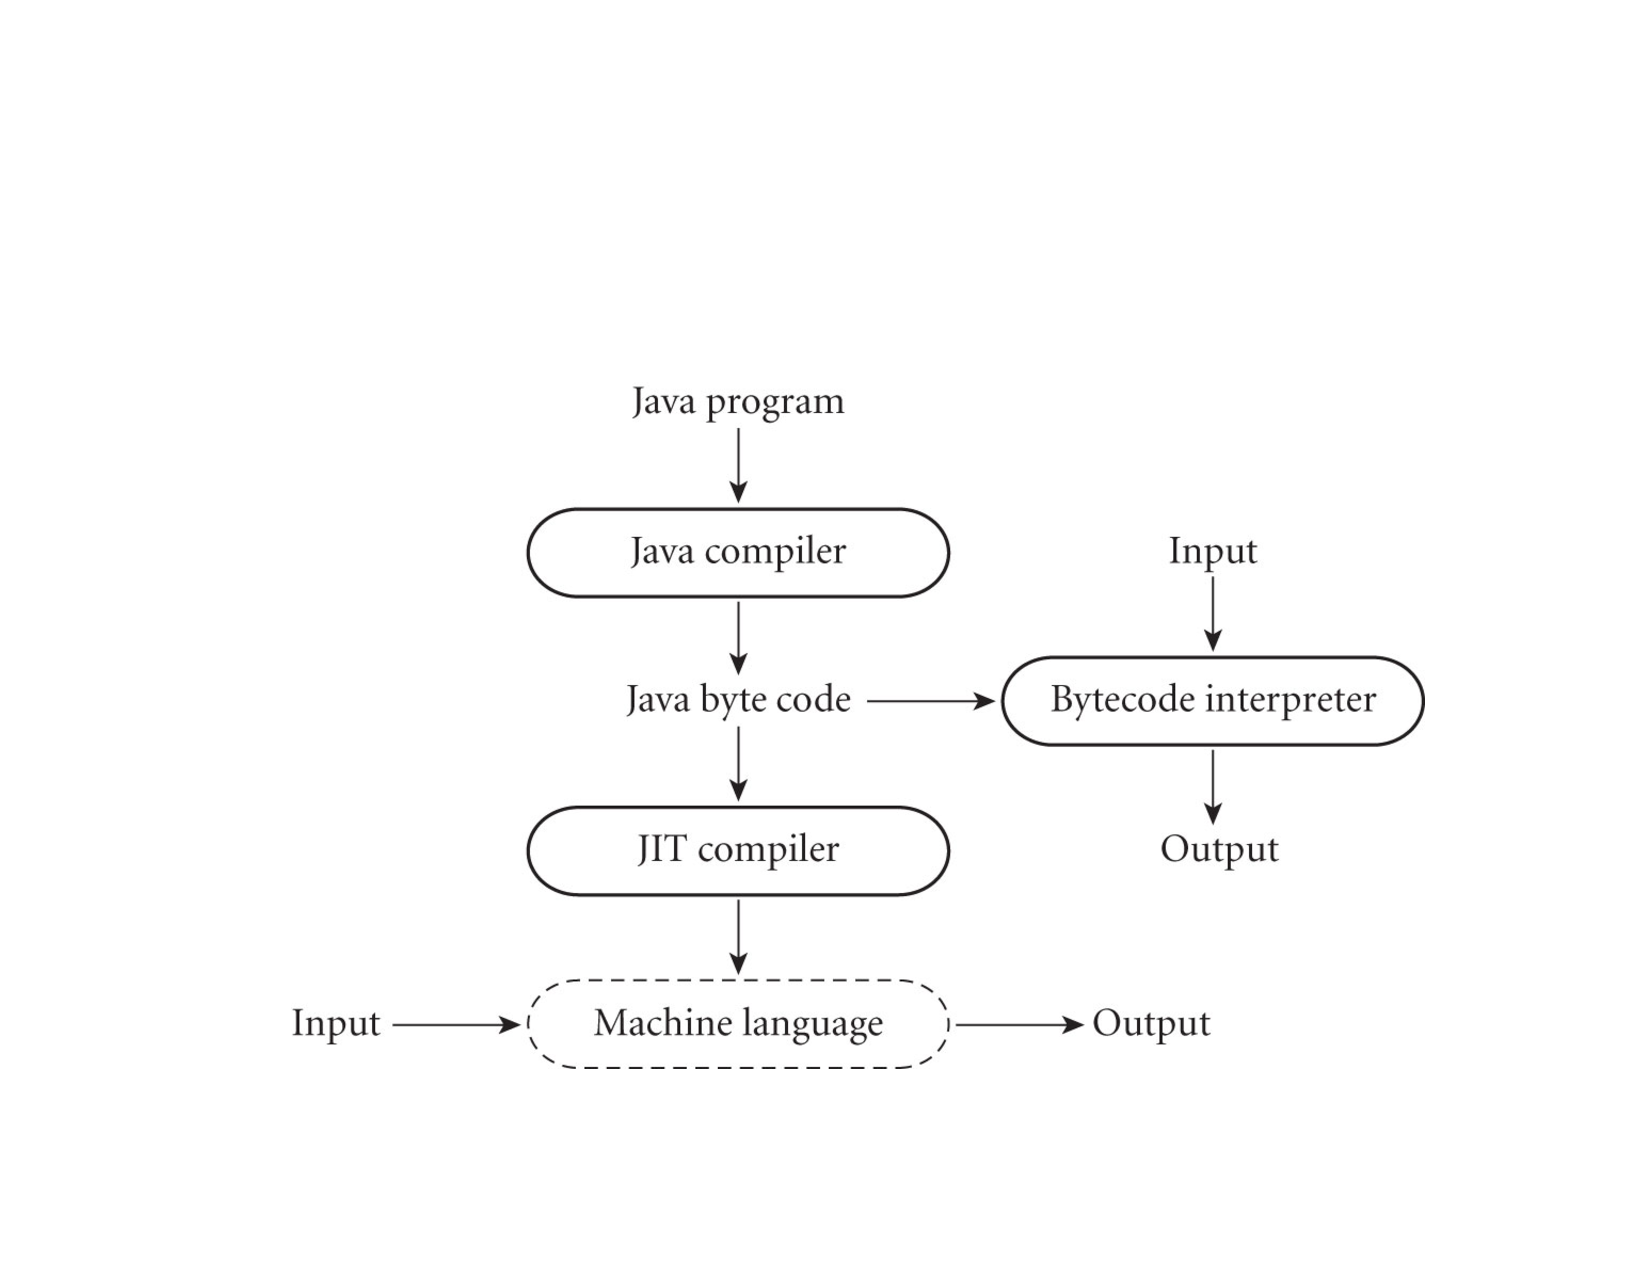
\includegraphics{images/javacompilation.pdf}}
\caption{Java compilation system}
\label{fig:javacompilation}
\end{figure}


Manually transforming programs is tedious and error-prone, because people make mistakes when manipulating code to enforce the explicit or implicit transformation rules.
Various automatic systems have been built to transform programs in a mechanic way. Such systems are built for different purposes. For instance, a source-to-source compiler translates programs from one programming language to another language. Source code generation produces source code based on an ontological model, which defines the types, properties, and interrelationships of entities. 
Many systems guarantee that each transformed program is semantically equivalent to the original program, while other systems do not preserve such semantic equivalence while transforming code. In this section, we will first overview various methods, techniques, and tools to automate source-to-source program transformation (Section~\ref{sec:automated}), and then especially discuss refactoring---one kind of semantic-preserving transformation (Section~\ref{sec:refactoring}), and systematic editing---one kind of transformation that does not preserve semantics (Section~\ref{sec:sysedit}).



\subsubsection{Perfective Changes} 
\todo{Miryung: Write the following paragraph more broadly. refactoring is a special category of automated transformation: refactoring practices (kim et al., emerson murphy hill, ralph johnson) } 

Code refactoring is the process of restructuring source code without changing its external behaviors. It is usually applied to improve code readability or extensibility, or to reduce code complexity. 
Fowler et al.~defined a catalog of refactorings that developers can apply to improve their codebase in different ways~\cite{1999:RID}, although developers can also define and manually apply their own refactorings. Eclipse IDE also provides tool support to automate some of the refactorings mentioned in Fowler's catalog, such as \emph{Extract Method}, \emph{Pull up Method}, and \emph{Move Field}. Researchers proposed various approaches to automate refactoring or to complete the refactoring tasks initiated by developers~\cite{Griswold:1992,Balazinska1999,Dig:2009,Ge:2012,Chen:2013,Lee:2013,Tsantalis2013:icsm,Meng:2015,Kim:2016}.
\todo{Start from Bill Griswold and Okdype, Ralph Johnson} 

To ensure the semantic equivalence between programs that are before and after a predefined refactoring program transformation, automated tools always check some pre-conditions before applying the transformation, and may check some post-conditions after the transformation.
In this section, we will explain two refactoring tools with more details: Drag-and-Drop Refactoring (DNDRefactoring)~\cite{Lee:2013} and R3~\cite{Kim:2016}.

\todo{Miryugn to Na: we should discuss a survey of refactoring papers by Mens} 
\todo{Miryung to Na: DND refactoring does not seem like a seminal paper. Reduce the example section on this more.} 
\paragraph{Drag-and-Drop Refactoring.} Prior research identified at least three dominant usability problems when using automated refactoring tools~\cite{OConnor:2005,Mealy:2007,Parnin:2008,Murphy-Hill:2008,Murphy-Hill:2011,Vakilian:2012}. First, programmers have trouble identifying opportunities for using the tools. Second, programmers have difficulty invoking the right refactoring from a lengthy menu of available refactorings. Third, programmers find it complicated to properly configure refactoring dialogs. DNDRefactoring was proposed to facilitate automated refactoring by allowing programmers to apply refactorings through direct manipulation on program elements, including variables, expressions, statements, and methods, in the IDE. In this way, developers do not need menus or dialogs to specify what refactoring to apply or how to apply those refactorings. Instead, DNDRefactoring can automatically infer such information by monitoring the selection and drag-and-drop operations of developers.

Figure~\ref{fig:dnd} presents two scenarios where DNDRefactoring automates refactorings based on the gestures of developers in Eclipse IDE. As shown in Figure~\ref{fig:dnd} (a), when developers select a code snippet in an existing method \codefont{bar(...)}, and then drag-and-drop the snippet to a location outside \codefont{bar(...)}, DNDRefactoring automates the \emph{Extract Method} refactoring by creating a new method \codefont{extracted(...)}, which takes in one parameter: \codefont{name}. In this process, no menu or configuration dialog is needed, because the tool can infer developers' refactoring intent, and decide all detailed information required for the refactoring, such as the method name, the method body, and the code location where to place the new method. Figure~\ref{fig:dnd} (b) shows another scenario. When developers manually select the \codefont{InnerClass}, a class declared inside another class \codefont{OuterClass}, and then drag-and-drop the class to a package \codefont{pkg}, DNDRefactoring infers that developers want to extract the type and create a new Java file. Therefore, it generates a Java file InnerClass.java to hold all implementation of \codefont{InnerClass}.

\begin{figure}
\centering
\scalebox{0.5}{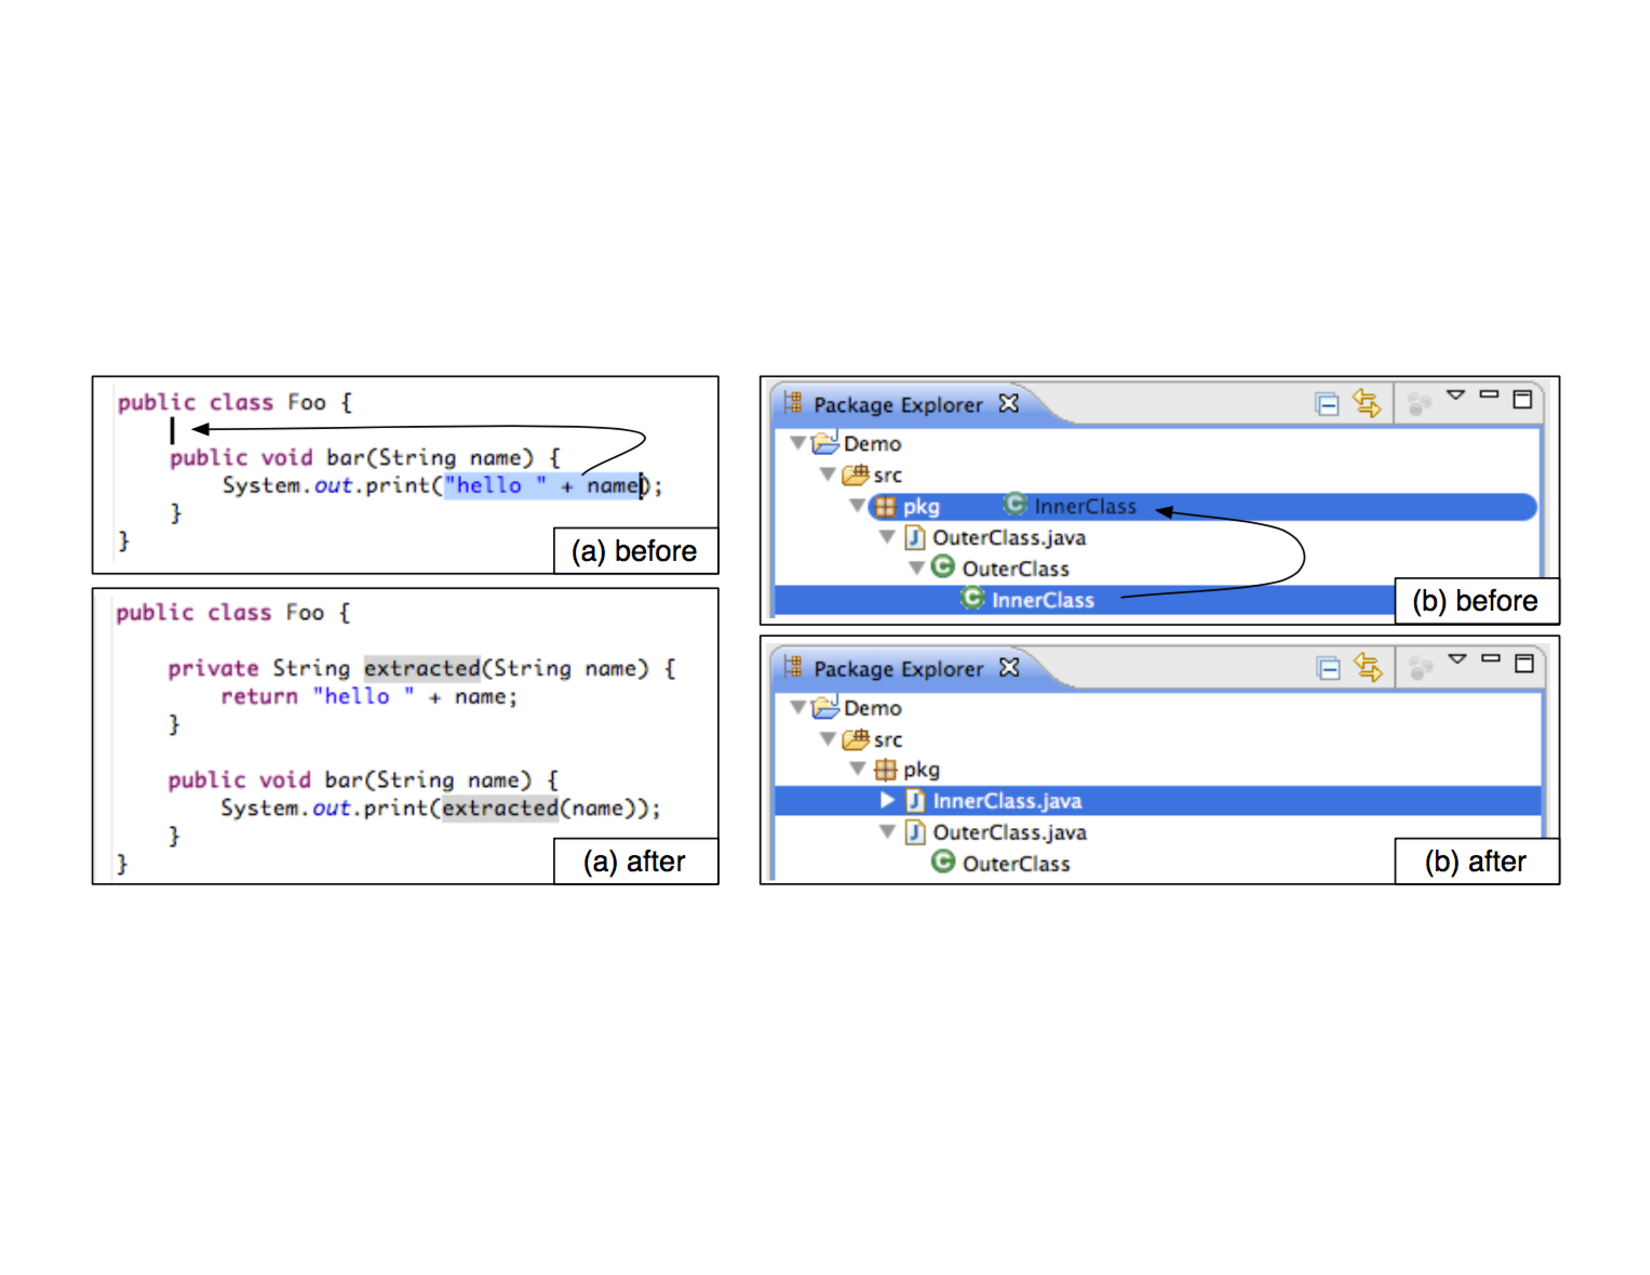
\includegraphics{images/DNDRefactoring.pdf}}
\caption{DNDRefactoring: Drag-and-drop gestures in (a) Java editor for Extract Method refactoring, and (b) Package Explorer for Extract Type to New File refactoring~\cite{Lee:2013}.}
\label{fig:dnd}
\end{figure}

Although DNDRefactoring demonstrated effectiveness in simplifying the application of automated refactorings, it still suffers from several limitations. First, not every refactoring can be conducted in a drag-and-drop manner. DNDRefactoring effectively supports move- and extract-based refactorings, but does not support \emph{Rename} refactoring. If developers want to rename a variable or a class, they cannot express that intent via selecting some text and moving it around with the cursor. Second, even for move- or extract- based refactorings, DNDRefactoring mainly works when the drag source and drop target elements are shown in the same screen. It does not work when these elements are located too far away to be presented in the same visual editor simultaneously. Third, DNDRefactoring does not allow users to freely configure refactoring details. For example, when users want to specify a meaningful name of an extracted method, with DNDRefactoring, they have no way to customize the information.

\todo{Miryung to Na. R3 does not seem like a seminal paper. I'd reduce the space allocation on this.} 
\paragraph{R3.} Compared with DNDRefactoring which improves the usability of Eclipse Refactoring with better UIs, R3 presents an alternative refactoring engine that works 10 times faster than Eclipse Refactoring. Specifically, R3 provides refactoring scripts as short Java methods, which enables users to easily define new refactorings. 
To speed up the application of refactorings, R3 first parses Java sources files, and builds a main-memory, non-persistent database to encode Java entity declarations (e.g., packages, class, methods), their containment relationships, and language features such inheritance and modifiers. By converting program Abstract Syntax Tree (AST) transformations to database queries and manipulations, R3 significantly reduces the runtime overhead of automating refactorings.


\begin{figure}
\centering
\scalebox{0.5}{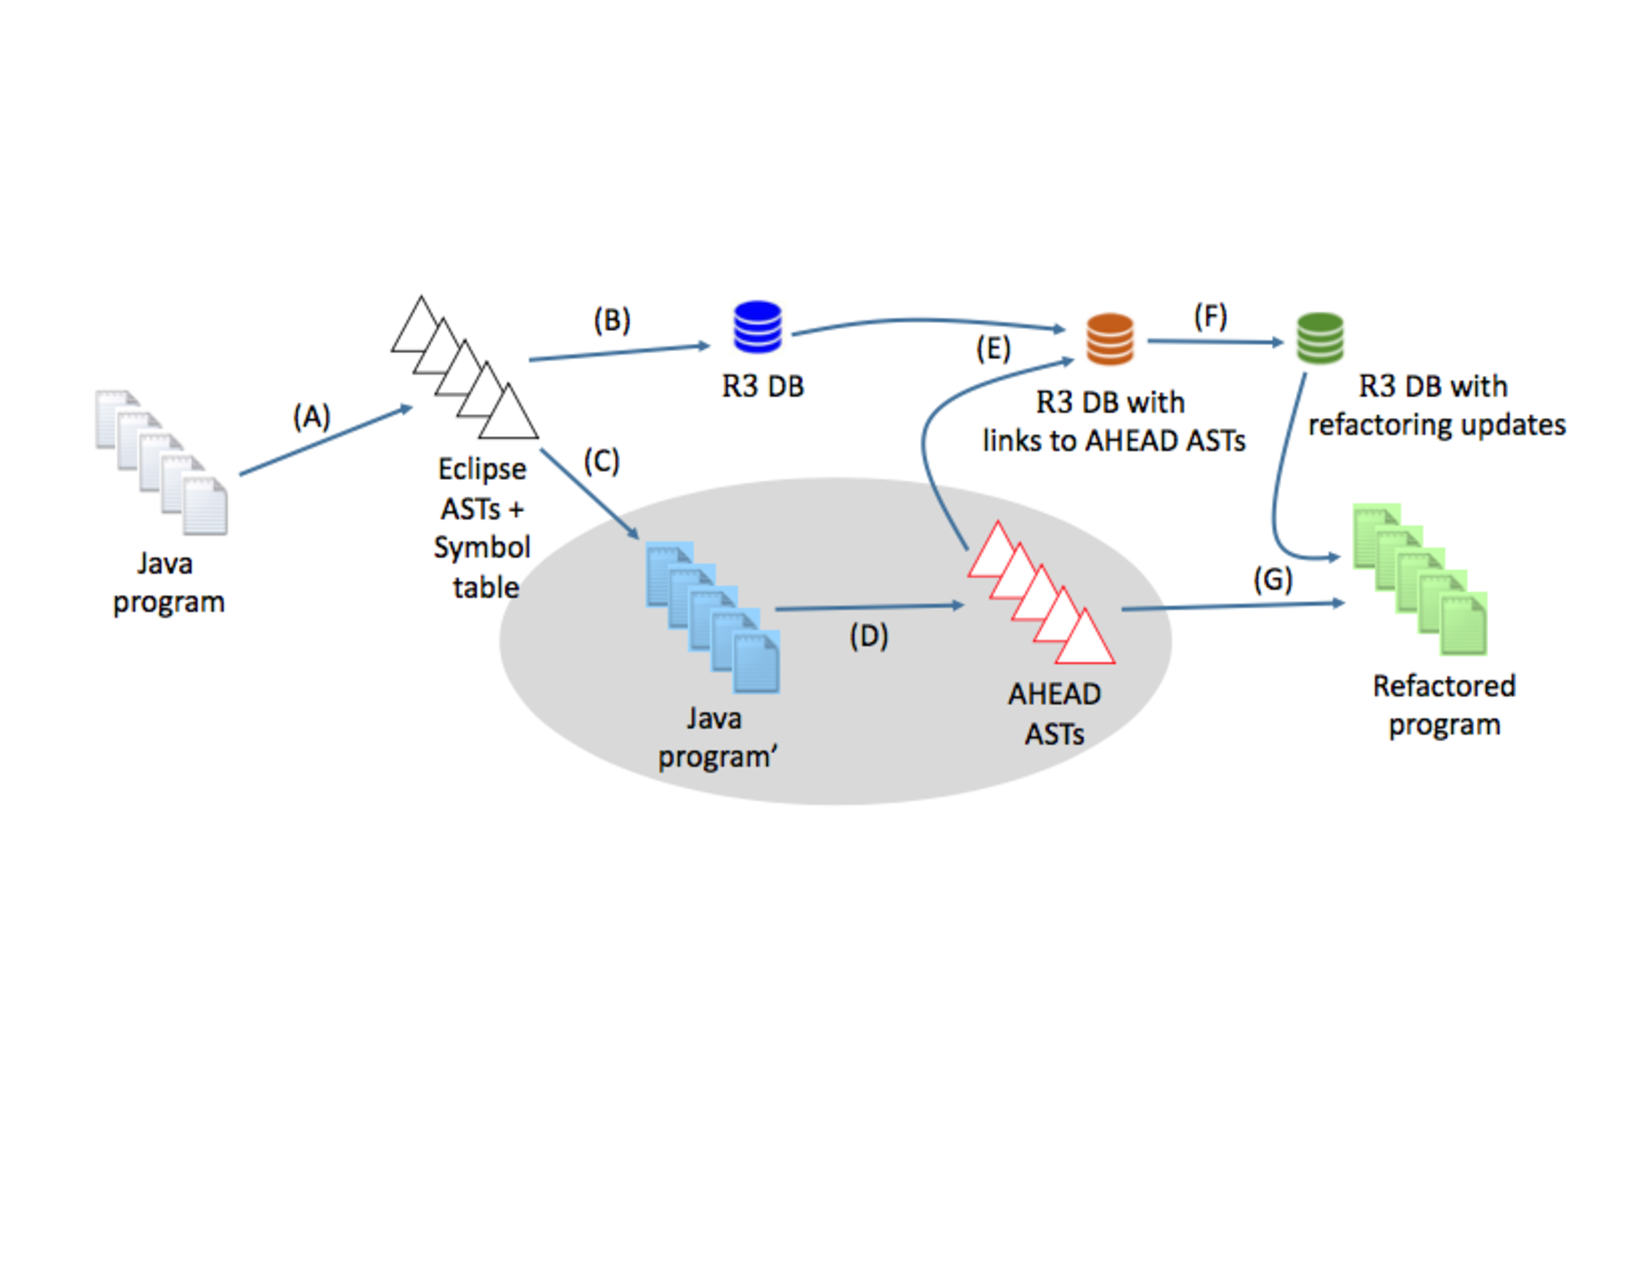
\includegraphics{images/r3overview.pdf}}
\caption{R3 pipeline~\cite{Kim:2016}.}
\label{fig:r3overview}
\end{figure}

Figure~\ref{fig:r3overview} presents the R3 pipeline, which has a series of stages (A)-(G) that map a target Java program (JDT project) on the left to a refactored program on the right. Stage (A) parses a Java program into ASTs with an Eclipse ASTParser. Stage (B) visits each generated AST to gather all Java entity-relevant information, and to save the information in R3 DB. To prepare program refactorings based on R3 DB, stage (C) generalizes the original program by replacing concrete entity information with abstract symbolic names, with each name corresponding to one concrete entity identifier kept in R3 DB. Stage (D) uses AHEAD~\cite{Batory:2003} to further parse the generalized program representation and create AHEAD ASTs. In Stage (E), tuples in R3 DB are doubly-linked to their AHEAD AST nodes, so that each pretty-printer of an AST node can reference the corresponding R3 tuple and vice versa. 

Stage (F) execute R3 refactorings. Unlike classical refactoring engines that modify Abstract Syntax Trees (ASTs), R3 refactorings modify only the database. For instance, if developers want to move a method from one class to another class, R3 does not directly move the method AST. Instead, it simply updates the method's database entry to have the new receiver type. With such information updates to the database, R3 can avoid repetitive AST manipulations. Finally, according to the updated entity information in R3 DB, stage (G) pretty-prints the source code, producing the resulting refactored program.

In addition to converting expensive AST manipulations to cheap database updates, R3 also precomputes the value of many properties of Java entities and saves those values in its database. Since these values can be used int the precondition checks of many refactoring tasks, keeping them in the database can avoid repetitive value computations, which can further reduce runtime overhead. R3 can well handle move- and rename-based refactorings, but does not support extract-based refactorings, because it does not store or modify statement-level or expression-level information in the database.  


\subsubsection{Corrective Changes} 
	- discuss literature on bug fixes  
	\todo{more empirical studies by S. Kim et al and T. Nguyen et al} 
	\todo{specialize bug fix techniques by Y.Y Zhou, S. Lu} 

\subsubsection{Additive Changes}
discuss literature on adding features, (systematic editing is a specialized technique for automated feature addition) source to source transformation 

\todo{add some literature on cross cutting changes. P. Tarr} 

\paragraph{Source to Source Transformation} 

\todo{perhaps reduce the space allocation on systematic editing a bit} 

\paragraph{Systematic Editing}
\label{sec:sysedit}
Systematic editing is the process of applying similar, but not necessarily identical, program changes to multiple code locations. Prior work shows that programmers apply systematic edits to either add features, fix bugs, or refactor code~\cite{Kim:2005,Kim:2009,Nguyen:2010}. Manually applying similar but different edits to multiple code locations is tedious and error-prone for two reasons. First, developers may forget to apply systematic edits to all program contexts where the edits are needed, committing errors of omission. Second, developers may apply edits inconsistently and thus introduce new bugs. To improve programmer productivity and software quality, several approaches~\cite{MKM2011,MKM2013,Rolim:2017} have been proposed to infer the general program transformation from one or more code change examples provided by developers, and then apply the transformation to other program contexts in need of similar changes. In this section, we will explain one approach with more details---SYDIT~\cite{MKM2011}, and briefly discuss another approach: LASE~\cite{MKM2013}.

\paragraph{SYDIT.} When developers want to change multiple code locations in similar but not identical ways, SYDIT requires developers (1) to modify one of these code locations and present it as a code change example, and (2) to manually specify the other locations to change similarly. By inferring a program transformation from the given example, SYDIT can apply the transformation to those locations and automate systematic editing accordingly.

\begin{figure}
\centering
\scalebox{0.45}{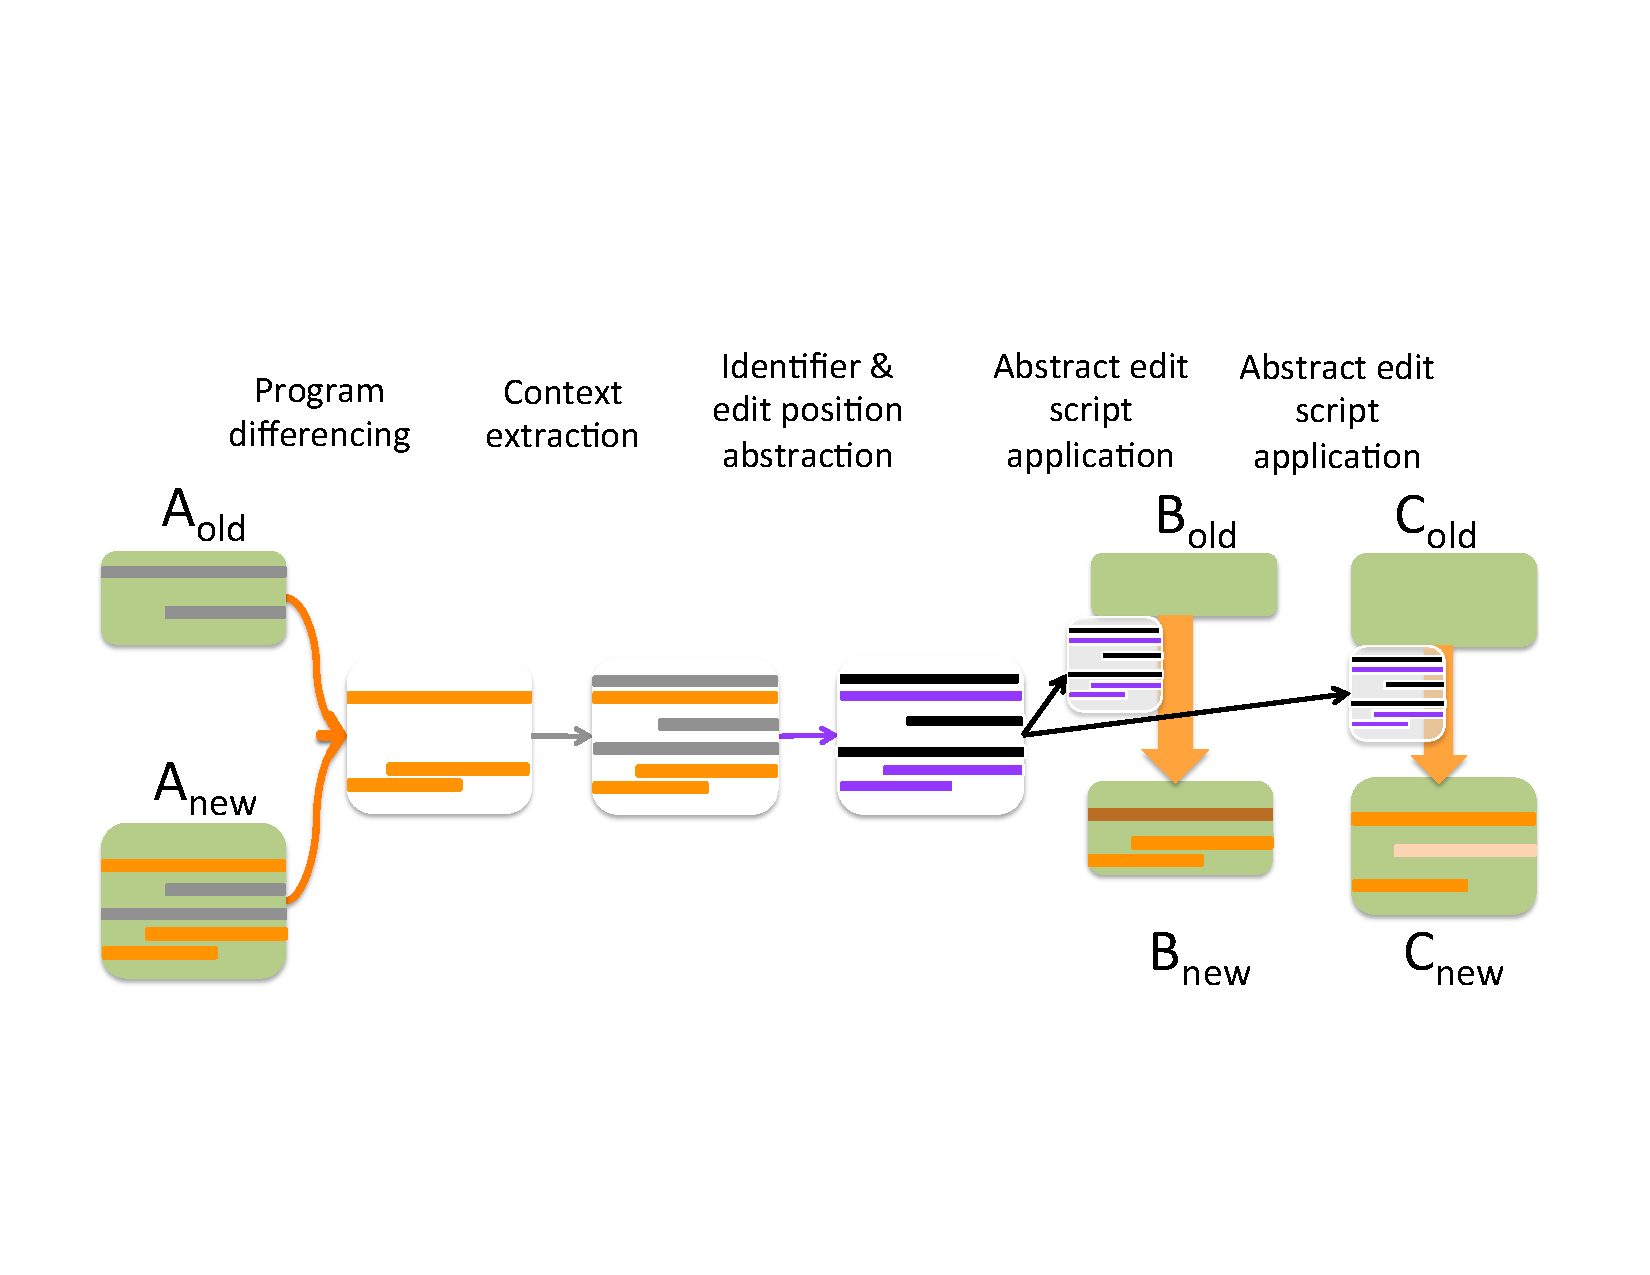
\includegraphics{images/syditoverview.pdf}}
\caption{SYDIT overview.}
\label{fig:syditoverview}
\end{figure}

As shown in Figure~\ref{fig:syditoverview}, suppose developers want to apply systematic edits to three methods: A, B, and C. Without any tool support, developers have to manually apply these similar but different edits to all three locations. With SYDIT, developers only need to (1) modify one location (e.g., A), and (2) manually specify the other locations to change (e.g., B and C). With the user input, SYDIT takes four steps to generalize and apply a program transformation. In the first step (program differencing), given the old and new version of method A, SYDIT first leverages ChangeDistiller~\cite{FWP2007} to compare the ASTs of both versions, and to extract changes as an AST edit script. The edit script may involve four types of statement-level edit operations: insert, delete, update, and move. To generalize the concrete edit script to a program transformation that is applicable to other program contexts, SYDIT needs to abstract the edit context and concrete identifiers. In step 2, SYDIT abstracts the edit context by identifying all unchanged code that is either control- or data-dependent on by the edited code, because such unchanged code manifests the semantic constraints those applied edits put on the program context. In step 3, SYDIT also abstracts the concrete identifiers used in the demonstrated edit so that the general program transformation is also applicable to code snippets that use different identifiers. Besides, SYDIT abstracts all edit operations' positions with respect to the extracted unchanged code, so that the inferred program transformation describes each edit operation within the edit-relevant context.
In this way, SYDIT derives an abstract, context-aware edit script from a given code change example.

In step 4, SYDIT concretizes the inferred program transformation to given code locations B and C, and applies the customized edits to suggest new versions of code. This step is the reverse process of the steps 1-3 mentioned above. With more details, given a code location to change (e.g., B), SYDIT first looks for any matching for the abstract edit context. If no matching is found, it indicates that similar changes should not be applied to the selected location, because the semantic constraints embedded in the abstract context are not satisfied. If one matching is found, SYDIT further concretizes the identifier usage and edit location information in the abstract script, creating a customized edit script applicable to the specific location. Finally, by modifying the code's AST based on the script, SYDIT produces a revised program for developers to review.

Although SYDIT can automate systematic editing in specified code locations, it always relies on users to manually pick those locations. In reality, finding code locations may be more challenging than applying the edits, especially when the codebase is large, and developers lack expertise of the project. Additionally, one code change example may not precisely characterize all program contexts which should be changed similarly. If the single example contains some edit-relevant context that is unique to the code location, SYDIT has no clue about how to only generalize the edit-relevant context which is commonly shared among all code locations.


\paragraph{LASE.} To facilitate systematic editing when developers cannot manually identify all code locations that should be changed similarly, LASE requires developers to provide at least two code change examples, from which it infers a general program transformation, and then leverages the transformation to both find other edit locations and suggest customized edits. 

\begin{figure}
\centering
\scalebox{0.35}{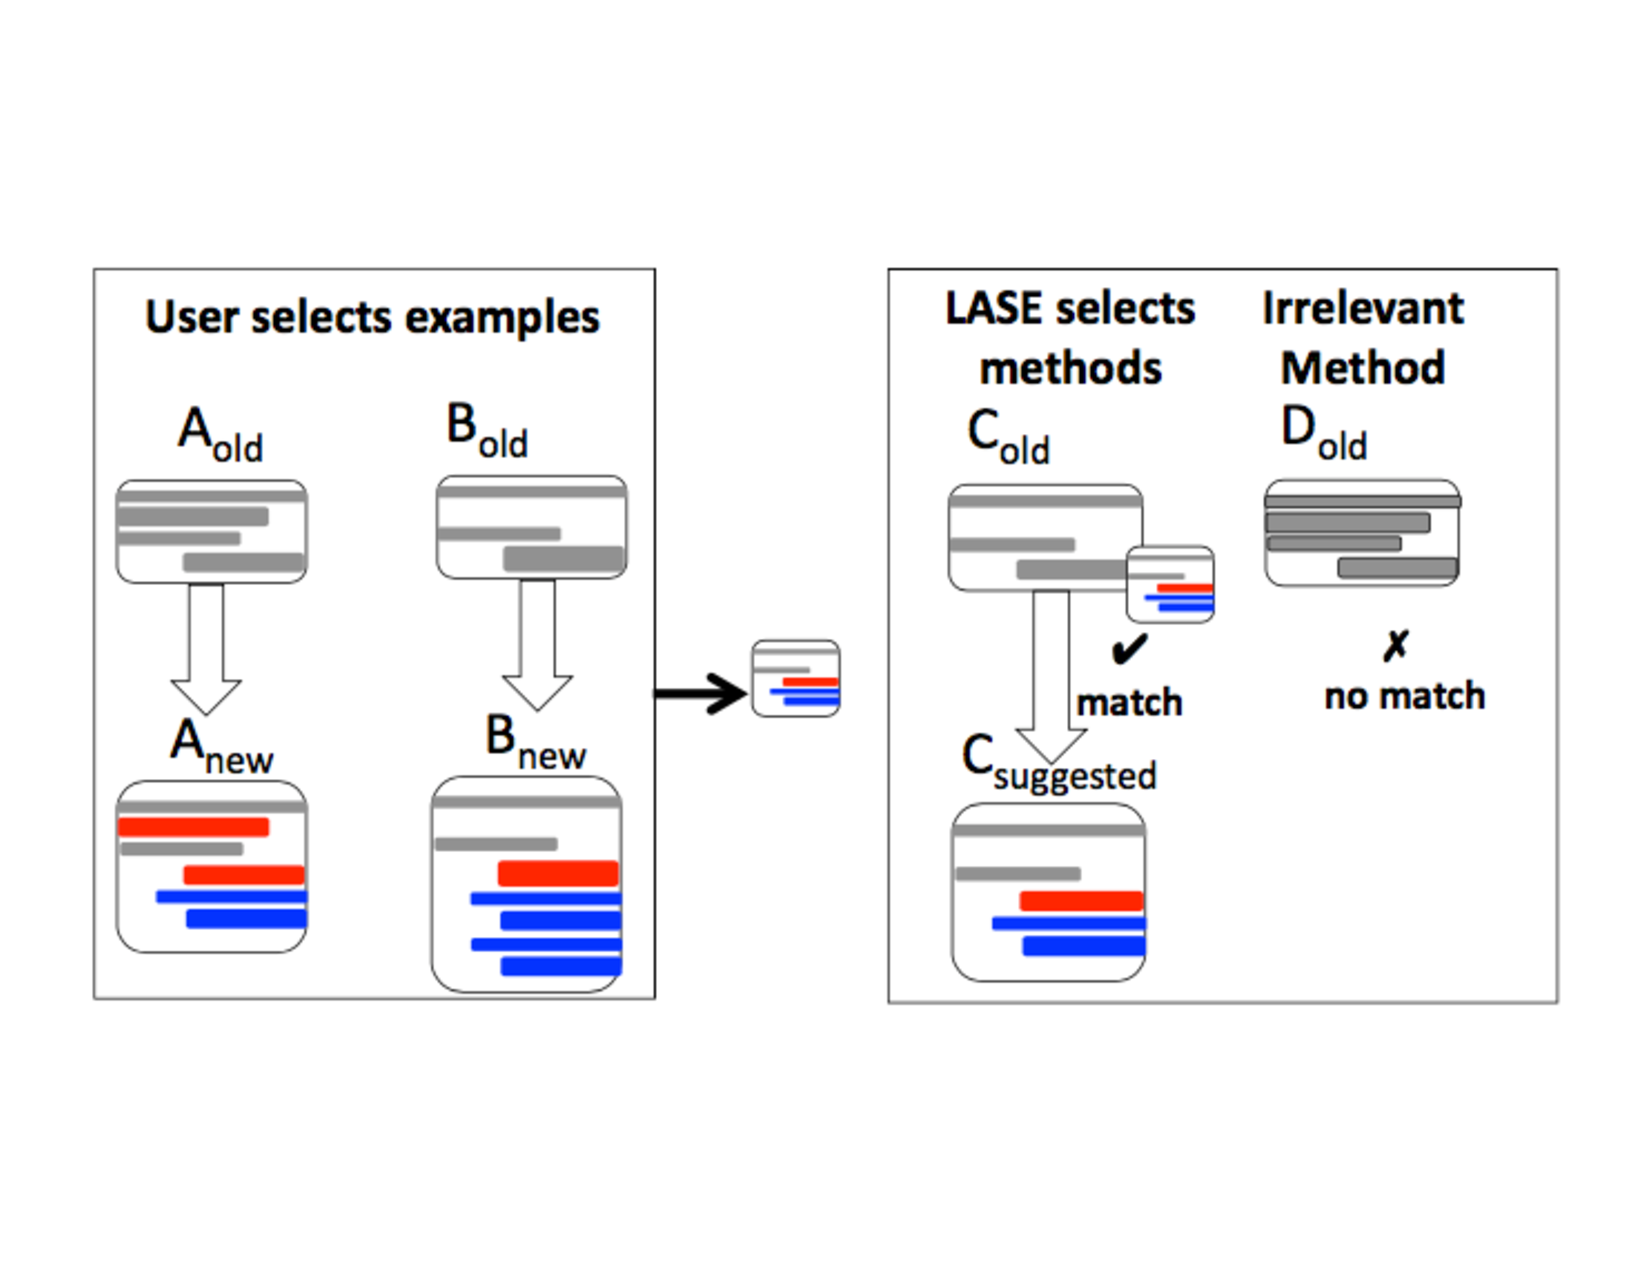
\includegraphics{images/laseoverview.pdf}}
\caption{LASE overview~\cite{MKM2013}.}
\label{fig:laseoverview}
\end{figure}

As shown in Figure~\ref{fig:laseoverview}, given two changed examples: A and B, LASE infers a general program transformation for each example, and then extracts the largest commonality between them in terms of edit operations, edit-relevant contexts, and identifier usage. In this way, LASE filters out any location-specific edit information, and only generalizes the program transformation that occurs multiple times. With such inferred program transformation, LASE attempts to establish matching between the abstract edit context and every method in the whole codebase. If a method contains a matching to the given context (e.g., C), LASE recommends the method as a candidate edit location, and suggests customized edits according to the matching information. If a method does not contain any matching to the given context (e.g., D), LASE considers the method as an irrelevant method to the systematic editing task.

\subsubsection{Porting programs to different languages} 
\subsubsection{Porting programs to different platforms} 

\subsection{Inspecting Program Changes}

\paragraph{Code Reviews Practices}
since code reviews is a common context where change inspection happens ( peter rigby)  code flow, collaborators in industry. generally starting from code review practices
\paragraph{Program Differencing} 
program differencing (going to back history of differencing, diff, AST diff, CFG diff, PDG diff.--- mention its symmetric problem of clone detection)
\paragraph{Techniques for Code Change Comprehension} 
go deeper for a few techniques that help with change comprehension: kim et al. critics, chris bird at MS


\subsection{Debugging and Testing Program Changes} 

\paragraph{Delta Debugging: Finding Code Changes Causing Errors}
\paragraph{Regression Testing} 
\paragraph{Change Impact Analysis} 

\section{Future Directions and Open Problems} 



\subsubsection*{Acknowledgments.} The heading should be treated as a
subsubsection heading and should not be assigned a number.

\section{The References Section}\label{references}
\bibliography{tianyi,mengna}
\bibliographystyle{abbrv}

\section*{Appendix} 
\end{document}
